\documentclass[11pt,a4paper,final]{article}

\usepackage[utf8]{inputenc}     % Codificación del archivo fuente en UTF8
\usepackage[T1]{fontenc}        % Incorpora fuente con acentos
\usepackage{amsmath}            % Amplía opciones para las ecuaciones
%\usepackage[margin=2cm]{geometry}

% -- Bibliografia --
%\usepackage[style=ieee,
%            backend=bibtex8,
%            maxcitenames=2,
%            mincitenames=1]
%            {biblatex}          % Control sobre las citas y referencias 
%  \addbibresource{Referencias.bib} % Archivo con las referencias
%\usepackage{url}                % Para incluir url clickeables

% -- Tuneando los captions --
\usepackage[margin=10pt,
            font=small,
            labelfont=bf,
            labelsep=endash]
            {caption}

% -- Tablas --
%\usepackage{booktabs}       % Decorado de tablas
%  \heavyrulewidth=1pt       % Lineas gruesas
%\usepackage{tabu}           % Permite control del ancho relativo entre columnas

% -- Figuras --
\usepackage{graphicx}		    % Permite incluir imágenes
  \graphicspath{{Figuras/}}	    % Ruta relativa donde buscar las imágenes
\usepackage[font=small,
            labelfont=bf, 
            subrefformat=parens]
            {subcaption}
            
% -- Incorporar imágenes de Matlab --
\usepackage{pgfplots}
\pgfplotsset{compat=newest} 
\pgfplotsset{plot coordinates/math parser=false}
\usepackage{tikz}
\usetikzlibrary{plotmarks} % para plotear las graficas que vienen de Matlab
            
%---------------------------------------------------------------------------------
% DEPRECATED COMMANDS
%---------------------------------------------------------------------------------  
\usepackage[spanish]{babel}     % Configura en modo español a muchas cosas
%\usepackage{amsfonts}
%\usepackage{amssymb}
\usepackage[babel,
            spanish=spanish]
            {csquotes}          % Comillas francesas en la bibliografia
%---------------------------------------------------------------------------------



\author{Sebastián R. Vanrell\\[3em]}
\title{{\Large Tópicos Selectos en Aprendizaje Maquinal}\\[3em]
       \textsf{Guía de Trabajos Prácticos Nº1}\\\bigskip
       \textsf{Algoritmos para Reconocimiento de Patrones}\\[3em]}
\date{Doctorado en Ingeniería\\\bigskip
      Facultad de Ingeniería y Ciencias Hídricas\\\bigskip
      Universidad Nacional del Litoral \\[5em]
      \today}

\usepackage{color}
\definecolor{lightgray}{gray}{0.5}
\setlength{\parindent}{0pt}

\begin{document}
\renewcommand{\tablename}{Tabla}

\maketitle
\newpage

\tableofcontents

\newpage

\section{Ejercicio 2}

Clasificación estadística de patrones.

\subsection{Ejercicio 2.1}

Sea un clasificador geométrico lineal definido por:
\begin{itemize}
\item $g_1(\mathbf{x}) = - x_1$ 
\item $g_2(\mathbf{x}) = x_1 + x_2 - 1$
\item $g_3(\mathbf{x}) = x_1 - x_2 - 1$
\end{itemize}
\begin{enumerate}
\item[a)] Calcule y grafique las fronteras y regiones de decisión.
\end{enumerate}

Para calcular las fronteras de decisión desarrollo las siguientes inecuaciones:
\begin{align*}
g_1(\mathbf{x}) &> g_2(\mathbf{x})   &  g_1(\mathbf{x}) &> g_3(\mathbf{x})  &  g_2(\mathbf{x}) &> g_3(\mathbf{x}) \\
- x_1           &> x_1 + x_2 - 1     &  - x_1           &> x_1 - x_2 - 1    &  x_1 + x_2 - 1   &> x_1 - x_2 - 1   \\
  x_2           &< - 2 x_1 + 1       &  x_2             &> 2 x_1 + 1        &  x_2             &> 0
\end{align*}

Para graficar las regiones de decisión (Figura \ref{ejercicio21}) considero que:
\begin{itemize}
\item $\mathbf{x} \in C_1 \;\; \mathrm{si} \;\; [g_1(\mathbf{x}) > g_2(\mathbf{x})] \wedge  [g_1(\mathbf{x}) > g_3(\mathbf{x})]$

\item $\mathbf{x} \in C_2 \;\; \mathrm{si} \;\; [g_2(\mathbf{x}) > g_1(\mathbf{x})] \wedge  [g_2(\mathbf{x}) > g_3(\mathbf{x})]$

\item $\mathbf{x} \in C_3 \;\; \mathrm{si} \;\; [g_3(\mathbf{x}) > g_1(\mathbf{x})] \wedge  [g_3(\mathbf{x}) > g_2(\mathbf{x})]$
\end{itemize}

\begin{figure}[h]
	\centering
	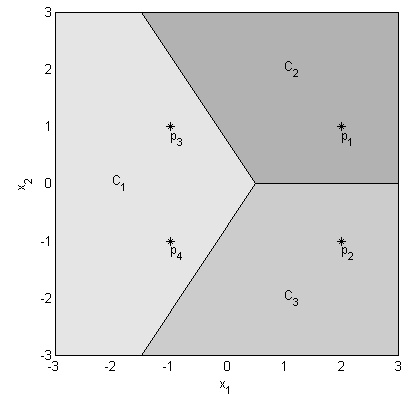
\includegraphics[width=.8\textwidth]{ejercicio21}
	\caption{Regiones y fronteras del clasificador geométrico lineal.}
	\label{ejercicio21}
\end{figure}

\begin{enumerate}
\item[b)] Clasifique los puntos (2,1); (2,-1); (-1,1); (-1,-1).
\begin{itemize}
\item $\mathrm{p_1}:\; (2,1) \in C_2$
\item $\mathrm{p_2}:\; (2,-1) \in C_3$
\item $\mathrm{p_3}:\; (-1,1) \in C_1$
\item $\mathrm{p_4}:\; (-1,-1) \in C_1$
\end{itemize}
\end{enumerate}

%\begin{par}
%Considere el sistema $H(z)=\frac{1-2z^{-1}+2z^{-2}-z^{-3}}{(1-z^{-1})(1-0.5z^{-2})(1-0.2z^{-3})}$
%\end{par}
%\begin{itemize}
%\setlength{\itemsep}{-1ex}
%   \item Dibuje el diagrama de ceros y polos. ¿Es estable el sistema?
%   \item Determine la respuesta al impulso del sistema
%\end{itemize}
%\begin{verbatim}
%clc; clear all; close all;
%
%num = [1 -2 2 -1];
%den = [1 -1.7 .8 -.1];
%H = tf(num,den);
%[ceros, polos] = zpkdata(H);
%
%hold on
%t = 0:0.01:2*pi;
%
%for j = 1:3
%    plot(real(ceros{1}(j)),imag(ceros{1}(j)),'o')
%    plot(real(polos{1}(j)),imag(polos{1}(j)),'x')
%    plot(cos(t),sin(t),'--')
%end
%grid on; axis tight; axis equal
%xlabel('Re(z)'); ylabel('Im(z)')
%title('Polos y ceros de H(z) en el plano z')
%legend('ceros','polos')
%hold off
%\end{verbatim}
%
%\begin{center}
%\includegraphics [width=4in]{GTP1ejercicio4_01.png}
%\end{center}
%\begin{par}
%Como no hay ningún polo fuera del círculo unitario. Entonces, el sistema es estable. El polo ubicado en 1+0i es cancelado por el cero de igual ubicación.
%\end{par}
%\begin{verbatim}
%N = 20;
%d = zeros(N,1); % Defino el impulso
%d(4) = 1;
%h = zeros(N,1); % Donde guardo la respuesta al impulso
%
%for n = 4:N
%    h(n) =  1*d(n) - 2*d(n-1) + 2*d(n-2) - 1*d(n-3) +...
%            1.7*h(n-1) - 0.8*h(n-2) + 0.1*h(n-3);
%end
%
%subplot(2,1,1)
%stem(1:N,d)
%xlabel('n'); ylabel('d(n)')
%title('Impulso aplicado en n=4')
%subplot(2,1,2)
%stem(1:N,h)
%xlabel('n'); ylabel('h(n)')
%title('Respuesta al impulso d(n), en n=4')
%\end{verbatim}
%
%\begin{center}
%\includegraphics [width=\textwidth]{GTP1ejercicio4_02.png}
%\end{center}
%\begin{par}
%La respuesta al impulso es finita, lo que nuevamente poné en evidencia la estabilidad del sistema.
%\end{par}
%
%
%
%\newpage
%
%\section{Ejercicio 5}
%
%\begin{par}
%Realice su propia implementación de las convoluciones lineal y circular mediante la utilización de ciclo \texttt{for}. Compare los resultados con la función \texttt{conv}.
%\end{par}
%\begin{verbatim}
%clear all; close all; clc
%
%h = [2 1 0.5 0];
%x = [0 1 2 2];
%
%convMatlab = conv(h,x);
%convLineal = convLineal(h,x);
%convCircular = convCircular(h,x,4);
%cconvMatlab = cconv(h,x,4);
%
%subplot(2,2,1)
%stem(convLineal)
%grid on;
%xlabel('n'); ylabel('y(n)')
%title('convLineal')
%
%subplot(2,2,3)
%stem(convMatlab)
%grid on;
%xlabel('n'); ylabel('y(n)')
%title('conv de Matlab')
%
%subplot(2,2,2)
%stem(convCircular)
%grid on;
%xlabel('n'); ylabel('y(n)')
%title('convCircular')
%
%subplot(2,2,4)
%stem(cconvMatlab)
%grid on;
%xlabel('n'); ylabel('y(n)')
%title('cconv de Matlab')
%\end{verbatim}
%
%\begin{center}
%\includegraphics [width=.8\textwidth]{GTP1ejercicio5_01.png}
%\end{center}
%
%Los resultados obtenidos son iguales a los de las funciones propias de Matlab.
%
%\subsection*{convLineal.m}
%
%\color{lightgray} \begin{verbatim}
%1     function y = convLineal(x,h)
%2     %CONVLINEAL convolucion lineal implementada con fors
%3     % y = convLineal(x,h)
%4     % x es la entrada
%5     % h la respuesta al impulso
%6     
%7     Nx = length(x);
%8     Nh = length(h);
%9     N =  Nx + Nh - 1; % Tamanio total del vector convolucion
%10    y = zeros(1,N);
%11    
%12    % invierte h y lo va desplazando hacia la derecha
%13    for n = 1:N
%14        jmin = max(n-Nh+1,1); % asegura no pasarse del ultimo elemento de h
%15        jmax = min(n,Nx);     % asegura no pasarse del ultimo elemento de x
%16        for j = jmin:jmax
%17            y(n) = y(n) + x(j)*h(n - j + 1);
%18        end
%19    end
%20    
%21    end
%22    
%
%\end{verbatim} \color{black}
%    
%
%\subsection*{convCircular.m}
%
%        \color{lightgray} \begin{verbatim}
%1     function y = convCircular( a, b, N)
%2     %CONVCIRCULAR convolucion circular implementada con fors
%3     % y = convCircular( a, b )
%4     % a es un vector
%5     % b es otro vector
%6     % N tamanio total del vector convolucion (modulo)
%7     
%8     y = zeros(1,N);
%9     
%10    % invierte a y lo hace rotar hacia la derecha en cada iteracion
%11    aaux = fliplr(a);
%12    for n = 1:N
%13        aaux = circshift(aaux,[0 1]);
%14        y(n) = aaux * b';
%15    end
%16    
%17    end
%18    
%
%\end{verbatim} \color{black}
%
%
%
%\newpage
%
%\section{Ejercicio 6}
%
%\begin{par}
%Dado el sistema 6*y[n]-4*y[n-1]+5*y[n-2]=x[n]-2*x[n-1]+x[n-2], inicialmente en reposo, obtenga la respuesta al escalón unitario mediante la ecuación en diferencias y luego compárela con la calculada mediante la sumatoria de convolución, para lo que debera encontrar previamente su respuesta al impulso.
%\end{par}
%\begin{verbatim}
%clear all; close all; clc
%
%% Defino un escalón a partir del instante n=3
%N = 30;
%escalon = [zeros(1,2) ones(1,N-2)];
%
%impulso = zeros(N,1); % Defino el impulso
%impulso(1) = 1;
%
%% Respuesta al impulso
%h = zeros(N,1);
%
%% Respuesta al escalón mediante ecuación en diferencias
%y1 = zeros(N,1);
%
%for n = 1:N
%    h(n)  =  impulso(n);
%    y1(n) =  escalon(n);
%    if n > 1
%        h(n)  =  h(n) - 2*impulso(n-1) + 4*h(n-1);
%        y1(n) =  y1(n) - 2*escalon(n-1) + 4*y1(n-1);
%    elseif n > 2
%        h(n)  =  h(n) + impulso(n-2) - 5*h(n-2);
%        y1(n) =  y1(n) + escalon(n-2) - 5*y1(n-2);
%    end
%    h(n)  = (1/6) * h(n);
%    y1(n) = (1/6) * y1(n);
%end
%
%% Respuesta al escalón mediante la convolución con la respuesta al impulso
%y2 = conv(escalon,h);
%
%subplot(5,1,1)
%stem(escalon); axis tight
%title('Escalon')
%xlabel('n'); ylabel('y(n)')
%
%subplot(5,1,2)
%stem(impulso); axis tight
%title('Impulso')
%xlabel('n'); ylabel('d(n)')
%
%subplot(5,1,3)
%stem(h); axis tight
%title('Respuesta al impulso')
%xlabel('n'); ylabel('h(n)')
%
%subplot(5,1,4)
%stem(y1); axis tight
%title('Por diferencias')
%xlabel('n'); ylabel('h(n)')
%
%subplot(5,1,5)
%stem(y2); axis tight
%title('Por convolucion')
%xlabel('n'); ylabel('h(n)')
%
%error = norm( y2(1:length(y1)) - y1)
%\end{verbatim}
%
%        \color{lightgray} \begin{verbatim}
%error =
%
%   2.0874e-16
%
%\end{verbatim} \color{black}
%    
%\begin{center}
%\includegraphics [width=\textwidth]{GTP1ejercicio6_01.png}
%\end{center}
%\begin{par}
%La respuesta al escalón obtenida por medio de la ecuación en diferencias es equivalente a los primeros N elementos de la respuesta obtenida por convolución. Esto último se puede corroborar con el cálculo de la norma del error donde su valor es del orden de 1x10\^{}-16 (error númerico)
%\end{par} \vspace{1em}
%
%
%
%\newpage
%\section{Ejercicio 7}
%
%\begin{par}
%Defina 3 señales cualesquiera y muestre numéricamente las siguientes propiedades.
%\end{par}
%\begin{verbatim}
%clear all; close all; clc
%
%t = 0:.01:1;
%x = sin(2*pi*t);
%y = randn(1,length(t));
%w = sawtooth(t);
%\end{verbatim}
%
%
%\subsection*{Conmutativa}
%
%\begin{par}
%$x*y = y*x$
%\end{par} \vspace{1em}
%\begin{par}
%Norma 2 del error entre lado derecho e izquierdo
%\end{par} \vspace{1em}
%\begin{verbatim}
%errorConmutativa = norm( conv(x,y) - conv(y,x) )
%\end{verbatim}
%
%        \color{lightgray} \begin{verbatim}
%errorConmutativa =
%
%   3.6955e-14
%
%\end{verbatim} \color{black}
%    
%
%\subsection*{Asociativa}
%
%\begin{par}
%$x * (y * w) = (x * y) * w$
%\end{par} \vspace{1em}
%\begin{par}
%Norma 2 del error entre lado derecho e izquierdo
%\end{par} \vspace{1em}
%\begin{verbatim}
%errorAsociativa = norm( conv(x,conv(y,w)) - conv(conv(x,y),w) )
%\end{verbatim}
%
%        \color{lightgray} \begin{verbatim}
%errorAsociativa =
%
%   1.1674e-12
%
%\end{verbatim} \color{black}
%    
%
%\subsection*{Distributiva con respecto a la suma}
%
%\begin{par}
%$x * (y + w) = (x * y) + (x * w)$
%\end{par} \vspace{1em}
%\begin{par}
%Norma 2 del error entre lado derecho e izquierdo
%\end{par} \vspace{1em}
%\begin{verbatim}
%errorDistributiva = norm( conv(x,y+w) - (conv(x,y) + conv(x,w)))
%\end{verbatim}
%
%        \color{lightgray} \begin{verbatim}
%errorDistributiva =
%
%   1.0777e-13
%
%\end{verbatim} \color{black}
%    \begin{par}
%Los errores distintos de 0 son significativamente pequeños y se los puede considerar como 0 desde un punto de vista numérico.
%\end{par} \vspace{1em}
%
%
%
%\newpage
%\section*{Ejercicio 8}
%
%\begin{par}
%Discretice una señal sinusoidal con frecuencia 5 Hz. y duración 1 seg. Utilice las siguientes frecuencias de muestreo: 1000, 100, 25, 10, 4, 1 y 0,5 Hz. Grafique y analice el resultado en cada uno de los casos.
%\end{par}
%\begin{verbatim}
%clear all; close all; clc
%
%fo = 5;
%
%fms = [1000 100 25 10 4 1 0.5];
%
%for j = 1 : length(fms)
%    fm = fms(j);
%    dt = 1/fm;
%    t  = 0:dt:1;
%    senial = sin(2*pi*fo*t);
%
%    subplot(ceil(length(fms)/2),2,j)
%    plot(t,senial)
%    title(['Senoidal de 5 Hz muestrada a ' num2str(fm) ' Hz'])
%    ylabel('sin(t)')
%    xlabel('t')
%end
%\end{verbatim}
%
%\begin{center}
%\includegraphics [width=\textwidth]{GTP1ejercicio8_01.png}
%\end{center}
%\begin{par}
%A partir de las gráficas en las que se muestreó una señal senoidal de 5 Hz con distintas frecuencias de muestreo se concluye lo siguiente:
%\end{par} \vspace{1em}
%\begin{itemize}
%\setlength{\itemsep}{-1ex}
%   \item fm = 1000 Hz: presenta la morfología y suavidad esperada.
%   \item fm = 100 Hz: presenta la morfología y suavidad esperada.
%   \item fm = 25 Hz: presenta la frecuencia base pero pierde la morfología y suavidad de la senoidal.
%   \item fm = 10 Hz: la señal se distorsiona y atenúa enormemente. No es posible distinguir una frecuencia constante en el intervalo de tiempo observado. Prácticamente se anula la señal.
%   \item fm = 4 Hz: la señal presenta una falsa periodicidad de 1 Hz. Provocada por aliasing.
%   \item fm = 1 Hz: Se observa una señal constante, de dos muestras y de valor nulo.
%   \item fm = 0.5 Hz: se tiene una sola muestra. No hay señal.
%\end{itemize}
%
%
%
%\newpage
%\section*{Ejercicio 9}
%
%\begin{par}
%Discretice una señal sinusoidal con frecuencia 4000 Hz. y duración 2 seg., utilizando una frecuencia de muestreo de 129 Hz. Grafique el resultado y estime la frecuencia de la onda sinusoidal que se observa en la figura. Analice y obtenga conclusiones.
%\end{par}
%\begin{verbatim}
%clear all; close all; clc
%
%fo = 4000;   % Frecuencia fundamental de la senial
%fm = 129;    % Frecuencia de muestreo
%dt = 1/fm;   % Periodo de muestreo
%t  = 0:dt:2; % Tiempos
%
%senial = sin(2*pi*fo*t);
%
%plot(t,senial)
%title(['Senoidal de 4000 Hz muestrada a ' num2str(fm) ' Hz'])
%ylabel('sin(2*pi*4000*t)')
%xlabel('t')
%
%frecObservada = mod(4000,129)
%\end{verbatim}
%
%        \color{lightgray} \begin{verbatim}
%frecObservada =
%
%     1
%
%\end{verbatim} \color{black}
%    
%\begin{center}
%\includegraphics [width=4in]{GTP1ejercicio9_01.png}
%\end{center}
%\begin{par}
%A partir de la gráfica se estima que la frecuencia de la señal es 1 Hz. Como se sabe, esto no es correcto. La alteracion observada se debe a que el muestreo se hace con una frecuencia mucho menor a la fundamental de la señal. El comportamiento observado es explicado a partir del aliasing que ocurre en estas condiciones. frecObservada es la frecuencia que se observaría por aliasing (verificando la sospecha anterior).
%\end{par} \vspace{1em}
%
%
%\newpage
%\section*{Ejercicio 12}
%
%\begin{par}
%Aproxime una onda cuadrada mediante series seno de diferente cantidad de términos y discuta la relación entre el resultado obtenido y el fenómeno de Gibbs.
%\end{par}
%\begin{verbatim}
%clear all; close all; clc
%
%fo = 1;      % Frecuencia fundamental de la onda cuadrada
%fm = 1000;   % Frecuencia de muestreo
%dt = 1/fm;   % Periodo de muestreo
%t  = 0:dt:2; % Tiempos
%N=40;
%enes = [1 3 10 40]; % Suma de n senos a graficar
%
%senial = square(2*pi*fo*t);
%aprox  = zeros(N,length(t));
%
%for k = 1:N
%    m = 2*k-1;
%    if k>1
%        aprox(k,:) = aprox(k-1,:);
%    end
%    aprox(k,:) = aprox(k,:) + (4/(pi*m)) * sin(2*pi*m*fo*t);
%end
%
%hold on
%plot(t,[senial; aprox(enes,:)])
%title('Senial cuadrada aproximada por series seno')
%ylabel('y(t)')
%xlabel('t')
%legend('Onda cuadrada','k=1','k=3','k=10','k=40')
%\end{verbatim}
%
%\begin{center}
%\includegraphics [width=\textwidth]{GTP1ejercicio12_01.png}
%\end{center}
%\begin{par}
%La convergencia de la serie seno de fourier falla en la discontinuidades de salto que presenta la onda cuadrada. A mayor cantidad de términos el error se reduce pero se manifiestan sobrepicos cerca de los puntos de saltos. Estos superan el 10\ensuremath{\backslash}\% del tamaño del salto. En el límite la serie converge a la función cuadrada tomando el valor medio para aquellos puntos que corresponden a un salto.
%\end{par} \vspace{1em}
%
%
%
%
%\newpage
%\section{Ejercicio 13}
%
%
%\begin{par}
%Genere una señal $s(t) = sin(2\pi f_1 t) + 4 sin(2\pi f_2 t)$, con $f_1 = 10$ y $f_2 = 20$ Hz, y obtenga su versión discreta s[n] con período de muestreo $T_m = 0,001$ seg. en el intervalo de tiempo t = [0...1) seg.
%\end{par}
%\begin{verbatim}
%clear all; close all; clc
%
%f1 = 10;        % Frecuencia de la primera senoidal
%f2 = 20;        % Frecuencia de la segunda senoidal
%Tm = .001;      % Período de muestreo
%fm = 1/Tm;      % Frecuencia de muestreo
%t  = 0:Tm:1-Tm; % Tiempos
%N  = length(t); % Cantidad de muestras
%df = fm/N;      % Resolución frecuencial
%f  = 0:df:fm-df;% Frecuencias
%
%senial = sin(2*pi*f1*t) + 4*sin(2*pi*f2*t);
%
%transformada = fft(senial);
%
%subplot(2,1,1)
%plot(t,senial)
%title(['Suma de senoidales en el tiempo'])
%ylabel('y(t)')
%xlabel('t')
%subplot(2,1,2)
%plot(f,abs(transformada))
%title(['Transformada de la suma de senoidales en frecuencia'])
%ylabel('Y(w)')
%xlabel('w')
%\end{verbatim}
%
%\begin{center}
%\includegraphics [width=4in]{GTP1ejercicio13_01.png}
%\end{center}
%\begin{par}
%Como era de esperar, se observa un pico en 10 Hz y otro en 20 Hz. La magnitud del pico en 20 Hz es 4 veces más grande que el de 10 Hz.
%\end{par} \vspace{1em}
%
%
%\subsection*{Verificando la relación de Parseval}
%
%\begin{par}
%Utilizo la norma 2 para calcular la energia
%\end{par} \vspace{1em}
%\begin{verbatim}
%energiaSenial = norm(senial)^2
%
%energiaTransf = (1/N)*norm(abs(transformada))^2
%\end{verbatim}
%
%        \color{lightgray} \begin{verbatim}
%energiaSenial =
%
%   8.5000e+03
%
%
%energiaTransf =
%
%        8500
%
%\end{verbatim} \color{black}
%    
%
%\subsection*{Realizando cambios a la senial original}
%
%\begin{itemize}
%\setlength{\itemsep}{-1ex}
%   \item Agregado de una constante igual a 4
%\end{itemize}
%\begin{verbatim}
%senial = sin(2*pi*f1*t) + 4*sin(2*pi*f2*t) + 4;
%transformada = fft(senial);
%
%subplot(2,1,1)
%plot(t,senial)
%title(['Suma de senoidales en el tiempo'])
%ylabel('y(t)')
%xlabel('t')
%subplot(2,1,2)
%plot(f,abs(transformada))
%title(['Transformada de la suma de senoidales en frecuencia'])
%ylabel('Y(w)')
%xlabel('w')
%\end{verbatim}
%
%\begin{center}
%\includegraphics [width=4in]{GTP1ejercicio13_02.png}
%\end{center}
%\begin{par}
%Se observa un pico a frecuencia f=0, que se corresponde con la constante agregada. La magnitud del valor de la transformada a f=0 es el doble que el correspondiente al pico de f=f2 debido a que la energía está concentrada sólo en f=0. En el caso de f2, la energía se reparte entre f=f2 y f=-f2.
%\end{par} \vspace{1em}
%\begin{itemize}
%\setlength{\itemsep}{-1ex}
%   \item Cambio de frecuencias: f1 = 10 Hz y f2 = 11 Hz.
%\end{itemize}
%\begin{verbatim}
%f1 = 10;
%f2 = 11;
%
%senial = sin(2*pi*f1*t) + 4*sin(2*pi*f2*t);
%transformada = fft(senial);
%
%subplot(2,1,1)
%plot(t,senial)
%title(['Suma de senoidales en el tiempo'])
%ylabel('y(t)')
%xlabel('t')
%subplot(2,1,2)
%plot(f,abs(transformada),'.')
%title(['Transformada de la suma de senoidales en frecuencia'])
%ylabel('Y(w)')
%xlabel('w')
%\end{verbatim}
%
%\begin{center}
%\includegraphics [width=4in]{GTP1ejercicio13_03.png}
%\end{center}
%\begin{par}
%Se observa un pico en f1 y otro en f2. Los valores de los coeficientes siguen la misma relación que las amplitudes de las senoidales que componen la señal.
%\end{par} \vspace{1em}
%\begin{itemize}
%\setlength{\itemsep}{-1ex}
%   \item Cambio de frecuencias: f1 = 10 Hz y f2 = 10.5 Hz.
%\end{itemize}
%\begin{verbatim}
%f1 = 10;
%f2 = 10.5;
%
%senial = sin(2*pi*f1*t) + 4*sin(2*pi*f2*t);
%transformada = fft(senial);
%
%subplot(2,1,1)
%plot(t,senial)
%title(['Suma de senoidales en el tiempo'])
%ylabel('y(t)')
%xlabel('t')
%subplot(2,1,2)
%plot(f,abs(transformada),'.')
%title(['Transformada de la suma de senoidales en frecuencia'])
%ylabel('Y(w)')
%xlabel('w')
%\end{verbatim}
%\begin{center}
%\includegraphics [width=4in]{GTP1ejercicio13_04.png}
%\end{center}
%\begin{par}
%En el dominio transformado, la resolucion frecuencial (1 Hz) no permite distinguir entre ambas senoidales, cuyas frecuencias se diferencian en 0.5 Hz. Esto es lo que provoca la aparición de colas en el entorno de 10 Hz
%\end{par} \vspace{1em}
%\begin{itemize}
%\setlength{\itemsep}{-1ex}
%   \item Cambio en el intervalo de tiempo de análisis: t=[0...0,72)
%\end{itemize}
%\begin{verbatim}
%f1 = 10;        % Frecuencia de la primera senoidal
%f2 = 20;        % Frecuencia de la segunda senoidal
%Tm = .001;      % Período de muestreo
%fm = 1/Tm;      % Frecuencia de muestreo
%t  = 0:Tm:0.72-Tm; % Tiempos
%N  = length(t); % Cantidad de muestras
%df = fm/N;      % Resolución frecuencial
%f  = 0:df:fm-df;% Frecuencias
%
%senial = sin(2*pi*f1*t) + 4*sin(2*pi*f2*t);
%transformada = fft(senial);
%
%subplot(2,1,1)
%plot(t,senial)
%title(['Suma de senoidales en el tiempo'])
%ylabel('y(t)')
%xlabel('t')
%subplot(2,1,2)
%plot(f,abs(transformada),'.')
%title(['Transformada de la suma de senoidales en frecuencia'])
%ylabel('Y(w)')
%xlabel('w')
%\end{verbatim}
%\begin{center}
%\includegraphics [width=4in]{GTP1ejercicio13_05.png}
%\end{center}
%\begin{par}
%En el dominio transformado, la resolución frecuencial (1.39 Hz) permitiría distinguir entre ambas senoidales, por tener 10 Hz de diferencia. Sin embargo, dado que en el eje de frecuencias no existen las frecuencias 10 o 20 Hz, la energía de las senoidales originales se reparte en las coeficientes correspondientes a frecuencias cercanas. Por ello es que se observan nuevamente las colas en torno a 10 y 20 Hz.
%\end{par} \vspace{1em}
%
%
%\newpage
%\section{Ejercicio 14}
%
%\begin{par}
%En la siguiente figura se observa el espectro de magnitud obtenido aplicando la TDF a una señal generada mediante la función $g(t) = \sin(2\pi f_1 t) + 4 \sin(2\pi f_2 t)$ y luego digitalizada.
%\end{par}
%\begin{verbatim}
%clear all; close all; clc
%\end{verbatim}
%\begin{par}
%Para resolver la pregunta pruebo con
%\end{par} \vspace{1em}
%\begin{verbatim}
%% Intervalo de tiempo durante la captura (en ms)
%Tlist  = 0.001 .* [249 498 993 498 993 124.5];
%% Frecuencia de muestreo
%fmlist = [512 128 128 256 128 1024];
%% Frecuencia de la primera senoidal
%f1list = [112 56 100 56 100 3872];
%% Frecuencia de la segunda senoidal
%f2list = [200 200 50 868 78 5520];
%
%j=1; % T=0.249, fm=512, f1=112, f2=200
%% for j = 1:length(Tlist)
%    T = Tlist(j);
%    fm = fmlist(j);
%    f1 = f1list(j);
%    f2 = f2list(j);
%
%    Tm = 1/fm;      % Período de muestreo
%    t  = 0:Tm:T;    % Tiempos
%    N  = length(t); % Cantidad de muestras
%    df = fm/N;      % Resolución frecuencial
%    f  = 0:df:fm-df;% Frecuencias
%
%    Nmuestras = fm*T    % Comprobando número de muestras
%    f1m = mod(f1,fm)/df % comprobando ubicacion de f1
%    f2m = mod(f2,fm)/df % comprobando ubicacion de f2
%
%    senial = sin(2*pi*f1*t) + 4*sin(2*pi*f2*t);
%    transformada = fft(senial);
%
%    subplot(2,1,1)
%    plot(t,senial)
%    title(['Suma de senoidales en el tiempo'])
%    ylabel('y(t)'); xlabel('t')
%
%    subplot(2,1,2)
%    stem(1:N,abs(transformada)); axis tight
%    title(['Transformada de la suma de senoidales en frecuencia'])
%    ylabel('Y(k)'); xlabel('k')
%    pause()
%% end
%\end{verbatim}
%
%        \color{lightgray} \begin{verbatim}
%Nmuestras =
%
%  127.4880
%
%
%f1m =
%
%    28
%
%
%f2m =
%
%    50
%
%\end{verbatim} \color{black}
%\begin{center}
%\includegraphics [width=4in]{GTP1ejercicio14_01.png}
%\end{center}    
%\begin{itemize}
%\setlength{\itemsep}{-1ex}
%   \item El conjunto de parámetros 2 es el único que no presenta un espectro similar. Inclusive la cantidad de muestras no coincide.
%   \item El resto de los conjuntos de parámetros podrían generar ese espectro debido a que es el espectro que les corresponde o por la presencia de aliasing.
%\end{itemize}
%
%
%
%\newpage
%\section{Ejercicio 15}
%
%\begin{par}
%Verifique las condiciones de aplicabilidad para la propiedad:
%\[x * y = \mathcal{F}^{-1}( \mathcal{F}(x) \mathcal{F}(y) )\]
%utilizando señales de \texttt{N} muestras y comparando los resultados de la convolución calculada mediante:
%\end{par} \vspace{1em}
%\begin{enumerate}
%\setlength{\itemsep}{-1ex}
%   \item la sumatoria de convolución con ciclos \texttt{for},
%   \item la función \texttt{conv},
%   \item la función \texttt{filter},
%   \item las funciones \texttt{fft} y \texttt{ifft} utilizadas directamente como lo indica la propiedad,
%   \item las funciones \texttt{fft} e \texttt{ifft} pero agregando \texttt{N - 1} ceros tanto a \texttt{x} como a \texttt{y}.
%\end{enumerate}
%\begin{verbatim}
%clear all; close all; clc
%
%% Defino dos señales de N muestras.
%N = 983;
%dt = 1/N;
%t = 0:dt:1-dt;
%x = sinc(2*pi*2*t);
%y = sawtooth(2*pi*3*t);
%
%% Calculo ambos lados de la igualdad mediante los métodos propuestos
%convFor = convLineal(x,y);
%convMatlab = conv(x,y);
%% filterMatlab = filter(x,1,y);
%invSinCeros = ifft(fft(x).*fft(y));
%
%xCeros = horzcat(x, zeros(1,length(y)-1)); % Agrego N-1 ceros a x
%yCeros = horzcat(y, zeros(1,length(x)-1)); % Agrego N-1 ceros a y
%
%invConCeros = ifft(fft(xCeros).*fft(yCeros));
%filterMatlab = filter(xCeros,1,yCeros);
%
%% Calculo la norma de los errores entre los resultados de los métodos
%dif21 = norm(convFor - convMatlab)
%dif23 = norm(filterMatlab - convMatlab)
%% dif24 = norm(invSinCeros - convMatlab) % distinto tamaño
%dif25 = norm(invConCeros - convMatlab)
%\end{verbatim}
%
%        \color{lightgray} \begin{verbatim}
%dif21 =
%
%   7.9916e-13
%
%
%dif23 =
%
%     0
%
%dif25 =
%
%   3.7920e-13
%
%\end{verbatim} \color{black}
%    \begin{par}
%Debido a que se superponen las curvas, algunas de ellas han sido desplazadas para poder observarlas. Los desplazamientos se indican en la leyenda.
%\end{par} \vspace{1em}
%\begin{verbatim}
%hold on
%plot(convFor,'b')
%% pause()
%plot(convMatlab+1,'g')
%% pause()
%plot(filterMatlab+2,'r')
%% pause()
%plot(invSinCeros,'k')
%% pause()
%plot(invConCeros+3,'m')
%legend('convLineal','conv + 1', 'filter con ceros + 2', 'ifft sin ceros',...
%       'ifft con ceros + 3')
%
%xlabel('n'); ylabel('y(n)')
%hold off
%\end{verbatim}
%\begin{center}
%\includegraphics [width=4in]{GTP1ejercicio15_01.png}
%\end{center}
%\begin{par}
%De los resultados obtenidos se concluye:
%\end{par} \vspace{1em}
%\begin{itemize}
%\setlength{\itemsep}{-1ex}
%   \item La convolución lineal con ciclos \texttt{for} y la implementada en Matlab no difieren en el resultado.
%   \item La utilización de la función \texttt{filter} será equivalente a utilizar la función \texttt{conv} si se agregan \texttt{N-1} ceros a \texttt{x} y \texttt{y}.
%   \item Si se agregan \texttt{N-1} ceros antes de aplicar la \texttt{fft} a \texttt{x} y \texttt{y} el resultado es equivalente a la convolución lineal. En cambio, si no se agregan los ceros la igualdad se pierde.
%\end{itemize}
%
%
%\newpage
%\section{Ejercicio 16}
%
%\begin{par}
%Realice un función para el cálculo y graficación de un espectrograma a partir de ciclos \texttt{for} y la transformada rápida de Fourier (\texttt{fft}). Utilice diferentes solapamientos y anchos de ventana para el análisis. Analice y discuta los resultados a la luz del principio de incertidumbre de Heisenberg.
%\end{par} \vspace{1em}
%\begin{verbatim}
%clear all; close all; clc
%
%f1 = 0;           % Frecuencia de la primera senoidal
%f2 = 200;         % Frecuencia de la segunda senoidal
%Tm = .001;        % Período de muestreo
%fm = 1/Tm;        % Frecuencia de muestreo
%t  = 0:Tm:1.5-Tm; % Tiempos
%N  = length(t);   % Cantidad de muestras
%df = fm/N;        % Resolución frecuencial
%f  = 0:df:fm-df;  % Frecuencias
%
%senial = chirp(t,f1,t(end),f2);
%
%
%subplot(2,2,1)
%plot(t,senial); ylim([-2 2])
%title(['Chirp lineal'])
%ylabel('y(t)')
%xlabel('t')
%
%subplot(2,2,2)
%tamVentana = 8;
%ventana = hann(tamVentana); % ventana de Hanning
%[s, fs, ts] = espectrograma(senial,fm,ventana,tamVentana);
%
%subplot(2,2,3)
%tamVentana = 64;
%ventana = hann(tamVentana); % ventana de Hanning
%[s, fs, ts] = espectrograma(senial,fm,ventana,tamVentana);
%
%subplot(2,2,4)
%tamVentana = 256;
%ventana = hann(tamVentana); % ventana de Hanning
%[s, fs, ts] = espectrograma(senial,fm,ventana,tamVentana);
%\end{verbatim}
%\begin{center}
%\includegraphics [width=\textwidth]{GTP1ejercicio16_01.png}
%\end{center}
%\begin{par}
%A partir de la función espectrograma construida se observa que al buscar resolución temporal (reduciendo el tamaño de las ventanas) la resolución frecuencial se ve afectada (aumentando las cajas en altura). Al contrario tambien, si se busca resolución frecuencial, se debe agrandar el tamaño de la ventana, lo que perjudica la resolución temporal.
%\end{par} \vspace{1em}
%
%
%\subsection*{espectrograma.m}
%
%\color{lightgray} \begin{verbatim}
%1     function [S, fs, ts] = espectrograma(x,fm,ventana,salto)
%2     %ESPECTROGRAMA 
%3     %   x es la señal
%4     %   fm es la frecuencia de muestreo
%5     %   ventana a utilizar para ventanear
%6     %   salto temporal para calcular la STFT
%7     
%8     N  = length(x);    % Cantidad de muestras
%9     Tm = 1/fm;         % Período de muestreo
%10    t  = 0:Tm:N*Tm-Tm; % Tiempos 
%11    % df = fm/N;       % Resolución frecuencial
%12    % f  = 0:df:fm-df; % Frecuencias
%13    
%14    medioAncho = ceil(length(ventana)/2);
%15    xlargo = [zeros(1,medioAncho) x zeros(1,medioAncho)];
%16    centro = 1 + medioAncho; % centro inicial
%17    
%18    % centro = ancho/2;  % centro de la primera ventana
%19    % salto = ancho - solapamiento; % salto para la proxima ventana
%20    
%21    ventanas = floor((N-1)/salto); % numero de ventanas
%22    
%23    S = zeros(medioAncho,ventanas); % Espectro, f en renglon y t por columnas
%24    ts = zeros(1,ventanas); % registro de tiempos para el espectrograma
%25    fs = zeros(1,medioAncho+1); % registro de frecuencias para el espectrograma
%26    
%27    for vent = 1:ventanas
%28        inicio = centro - medioAncho; % para segmentar xlarge
%29        final  = centro + medioAncho - 1; % para segmentar xlarge
%30        xloc = xlargo(inicio:final); % x local (recortado)
%31        
%32        Nx  = length(xloc); % Cantidad de muestras
%33        ts(vent)  = t(centro-medioAncho);  % Tiempos 
%34        df = fm/Nx;         % Resolución frecuencial
%35        fs  = 0:df:fm/2-df; % Frecuencias
%36        
%37        aux = abs(fft(xloc .* ventana'));
%38        S(:,vent) = aux(1:medioAncho);
%39        
%40        centro = centro + salto;
%41    end
%42    
%43    surf(ts,fs,S,'edgecolor','none')
%44    axis tight;
%45    view(0,90);
%46    title(['Espectrograma (tamVentana = ' num2str(medioAncho*2) ')'])
%47    xlabel('Tiempo (s)')
%48    ylabel('Frecuencia (Hz)')
%49    
%
%\end{verbatim} \color{black}
%
%
%\newpage
%\section{Ejercicio 17}
%
%\begin{par}
%Analice una señal senoidal cuya frecuencia crece linealmente desde cero hasta 8 veces la frecuencia de muestreo mediante la función anterior. Analice los resultados explicando claramente el fenómeno observado.
%\end{par}
%\begin{verbatim}
%clear all; close all; clc
%
%f1 = 0;         % Frecuencia inicial de la senoidal
%f2 = 8000;      % Frecuencia final de la senoidal
%Tm = .001;      % Período de muestreo
%fm = 1/Tm;      % Frecuencia de muestreo
%t  = 0:Tm:5-Tm; % Tiempos
%N  = length(t); % Cantidad de muestras
%df = fm/N;      % Resolución frecuencial
%f  = 0:df:fm-df;% Frecuencias
%
%senial = chirp(t,f1,t(end),f2);
%
%tamVentana = 64;
%ventana = hann(tamVentana); % ventana de Hanning
%paso = 1;
%[s, fs, ts] = espectrograma(senial,fm,ventana,1);
%\end{verbatim}
%\begin{center}
%\includegraphics [width=4in]{GTP1ejercicio17_01.png}
%\end{center}
%\begin{par}
%El espectrograma de una senoidal que crece linealmente desde frecuencia 0 hasta 8 veces la frecuencia de muestreo (fm) evidencia el fenómeno de aliasing. En los primeros instantes se observa un ascenso desde frecuencia 0 hasta fm/2. Este ascenso se condice con lo esperado y es correcto ya que la señal fue construida con ese comportamiento.
%\end{par} \vspace{1em}
%\begin{par}
%A continuación, el espectrograma identifica un descenso de la frecuencia. Esto no es real dado que la señal sigue aumentando su frecuencia. Lo que se observa entonces es el aliasing, donde las frecuencias por encima de fm/2 son reflejadas en frecuencias mas bajas. Así, los ascensos observados corresponden a frecuencias que pertenecen al rango (fm*k, (1+k)*fm/2) con k =0,1,...,7. De forma análoga, los descensos observados corresponden a frecuencias que pertenecen al rango (k*fm/2, k*fm) con k =1,2,...,8.
%\end{par} \vspace{1em}
%
%
%\newpage
%\section{Ejercicio 18}
%
%\begin{par}
%Realice el espectrograma de una señal senoidal cuya frecuencia crezca linealmente entre 100 y 200 Hz. Grafique el resultado con las escalas de tiempo y frecuencia adecuadas. Analice y discuta el resultado obtenido.
%\end{par}
%\begin{verbatim}
%clear all; close all; clc
%
%f1 = 100;       % Frecuencia inicial de la senoidal
%f2 = 200;       % Frecuencia final de la senoidal
%Tm = .001;      % Período de muestreo
%fm = 1/Tm;      % Frecuencia de muestreo
%t  = 0:Tm:1-Tm; % Tiempos
%N  = length(t); % Cantidad de muestras
%df = fm/N;      % Resolución frecuencial
%f  = 0:df:fm-df;% Frecuencias
%
%senial = chirp(t,f1,t(end),f2);
%
%tamVentana = 64;
%ventana = hann(tamVentana); % ventana de Hanning
%paso = 1;
%
%subplot(2,1,1)
%plot(t,senial)
%title(['Senoidal con f_ini=100 y f_fin=200 Hz'])
%ylabel('y(t)')
%xlabel('t')
%subplot(2,1,2)
%[s, fs, ts] = espectrograma(senial,fm,ventana,1);
%\end{verbatim}
%
%\begin{center}
%\includegraphics [width=4in]{GTP1ejercicio18_01.png}
%\end{center}
%\begin{par}
%El espectrograma de una senoidal que crece linealmente desde frecuencia 100 hasta 200 Hz evidencia dicha tendencia. Sin embargo, las frecuencias inicial y final no alcanzan a distinguirse debido al efecto de borde propio de utilizar las ventanas temporales. Así, del espectrograma se podría decir que la señal presenta una frecuencia escasamente superior a 100 Hz en un inicio y alcanza una frecuencia cercana a 200 Hz hacia el final de la captura.
%\end{par}

\end{document}